\chapter{Method}

\begin{comment}
Beskriv pipeline for å generere NeRFs

- Capture (video, image, polycam, etc.)
- Process (COLMAP, or direct extraction from e.g. Polycam)
    - Configuration of COLMAP
- Train (Different models)
    - Configuration of model
- Render (Real-time rendering vs. slow rendering)
- Evaluate (PSNR, SSIM, LPIPS)
- Export

- Pipelines created
    - Pipeline to test 
\end{comment}

\section{Nerfstudio}
With the magnitude of different published methods regarding NeRF, some with corresponding source code and some not, it's not trivial to compare them on self-captured data. In the experiments, I have leveraged an open-source project named Nerfstudio. It is an API that streamlines the creation, training, and visualization of NeRFs. The components that make up NeRFs are modularized in a way that allows interpretable implementation of different NeRF methods. In addition, it ships with implemented versions of some of the most important published methods to date for real-world captures; NeRF, mip-NeRF, and instant-NGP.

\section{Nerfacto}
Nerfstudio also provides its own method dubbed "Nerfacto". The method isn't published work, but leverages techniques from several other published methods which have proved to work well for real data captures. The techniques used in Nerfacto result in a method that strikes a great balance between quality and speed. Most of the techniques highlighted by Nerfacto have already been discussed in \autoref{chap:relatedwork}, but I'll recap and elaborate on a few here.

\textbf{Camera pose refinement} is a technique proposed for NeRFs on forward-facing scenes in \cite{wang_nerf--_2022}. It has later been built upon to support imperfect camera poses for full 3D scene representations in \cite{lin_barf_2021} and large, unbounded scenes in \cite{tancik_block-nerf_2022}. Pose refinement is a technique proposed to reduce the impact of imperfect camera poses. In NeRF, this can be done by treating the camera poses and intrinsics as learnable parameters and jointly optimizing them with the 3D scene representation, i.e. optimizing both the photometric loss and the corresponding camera poses. Pose refinement is a very effective measure to reduce cloudy artifacts and increase the sharpness and overall quality of the resulting 3D representation.

\textbf{Per image appearance conditioning} is a technique proposed for NeRFs in \cite{martin-brualla_nerf_2021} and later used in multiple implementations, including \cite{tancik_block-nerf_2022}. The appearance embedding is a vector in a low-dimensional space that is optimized jointly with the NeRF in order to allow the NeRF to process and represent 3D scenes with variable lighting, exposures, weather, and post-processing effects. In Nerfacto, the appearance embedding is a vector of size 32, which is concatenated with the viewing direction before it's passed through the MLP.
%The appearance embedding is concatenated with the viewing direction and passed through an MLP 

\textbf{Hash encodings} were proposed in \cite{muller_instant_2022}. This parametric encoding differs in how spatial data is represented. In the original NeRF paper, the location \textbf{x} is represented by a positional encoding. With the multiresolution hash encoding, the location \textbf{x} is represented in a hash table by a linear interpolation of its closest vertices at multiple resolutions. This parametric encoding has several advantages in terms of computational effectiveness, resulting in several magnitudes of increased training and inference speed. Although you impose a larger memory cost by allocating several hash tables, the number of required parameter-updates per backpropagation is severely reduced. In Nerfacto, 16 hash tables with $2^{19}$ rows, each storing a feature vector of size 2, are allocated. The subsequent MLP has a very low capacity, with only one hidden layer containing 64 neurons. An overview of the multiresolution hash encoding can be seen in \autoref{fig:instant-ngp-hash-encoding}.

\begin{figure}[h]
    \centering
    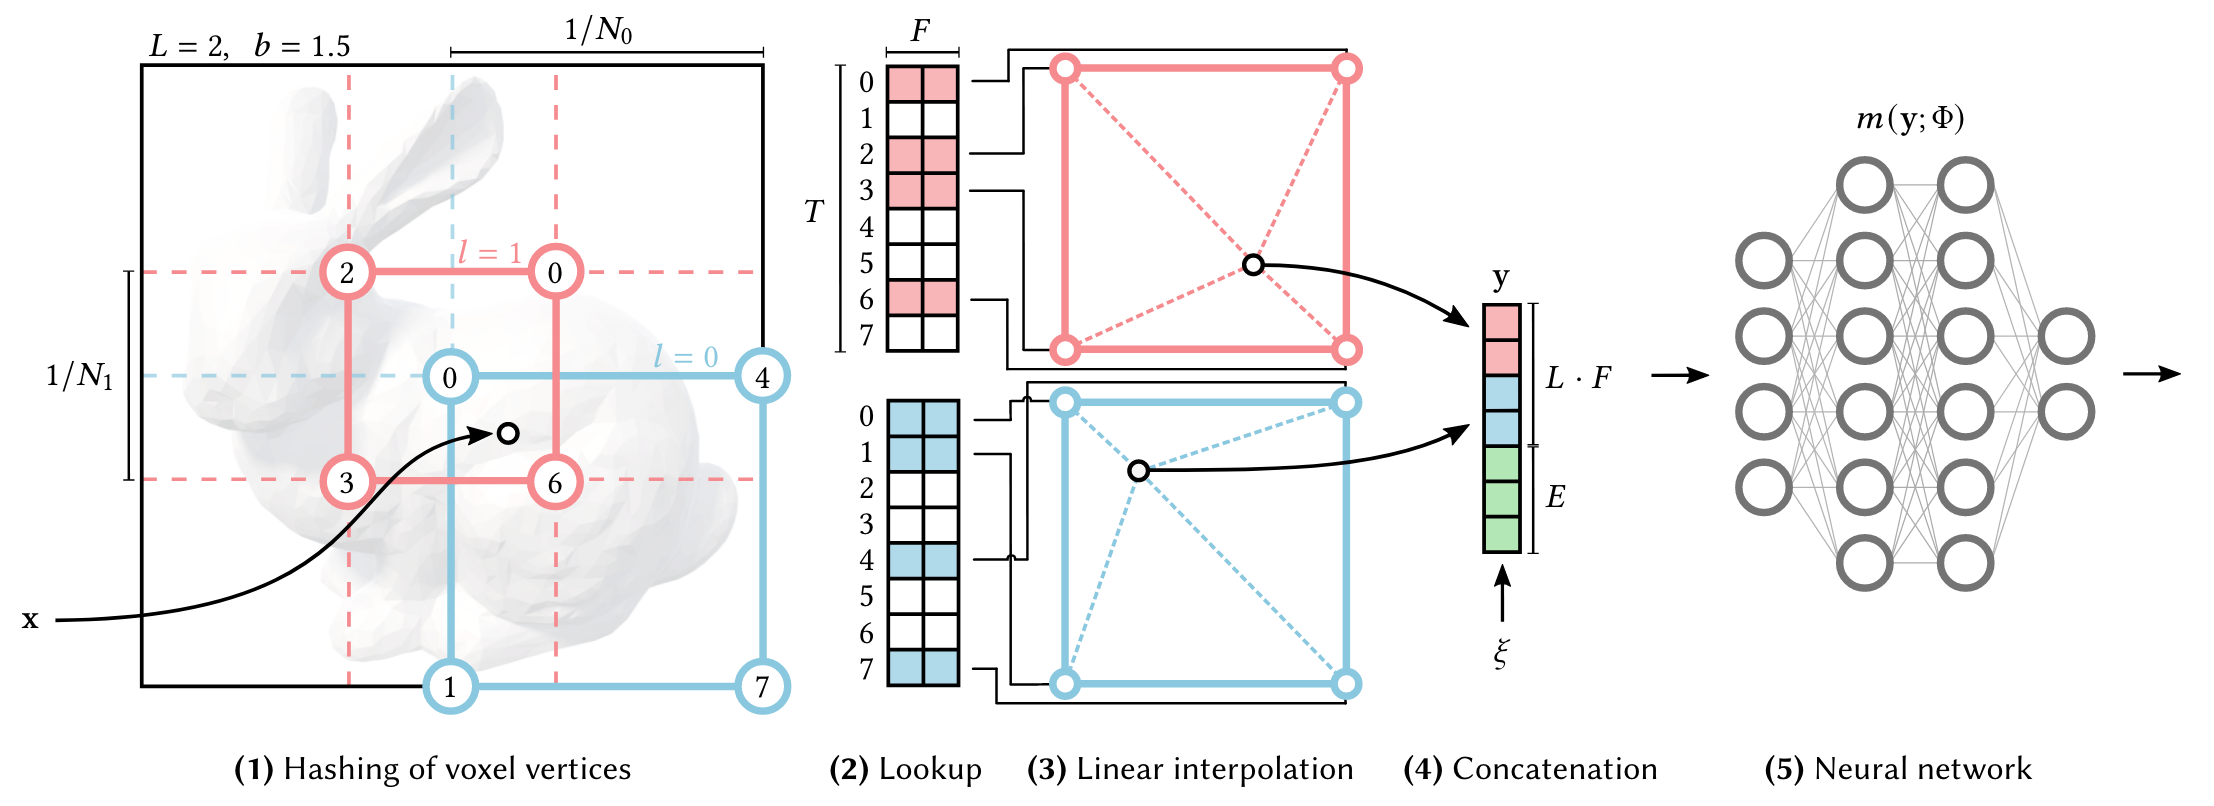
\includegraphics[width=1.0\textwidth]{figures/instant-ngp-hash-encoding.png}
    \caption{Illustration of the multiresolution hash encoding in 2D, Figure 3 \cite{muller_instant_2022}.}
    \label{fig:instant-ngp-hash-encoding}
\end{figure}

\textbf{Proposal sampling} is a sampling technique discussed in \autoref{sec:mipnerf360}. Nerfacto extends the proposal sampler used in mip-NeRF 360 by utilizing two density functions implemented as small fused-MLP with hash encodings \cite{muller_instant_2022}. This provides accurate and fast density estimations.

\textbf{Scene contraction} is yet another technique proposed in \cite{barronMipNeRF360Unbounded2022} and discussed in \autoref{sec:mipnerf360}.

%The only difference is essentially how spatial data is represented, i.e. parametric encoding. Instant-NGP encodes spatial data at multiple resolutions using hash tables, thereof the name multiresolution hash tables. During backpropagation, the MLP's weights and the feature vectors in the hash tables are both updated.
%In a fully connected MLP, every weight and bias must be updated on back-propagation. With parametric encodings, only a very small number of feature vectors must be updated. Also, by reducing the size of the MLP, such parametric models can be trained to convergence much faster without sacrificing approximation quality. You trade a larger memory footprint by allocating hash tables, but in return you have to update a far lower number of trainable parameters per back-propagation, leading to an increased training and inference speed.

%In instant-NGP, the max entries per hash table are $2^{24}$ and the default number of resolution levels is 16. This results in a memory allocation of $2^{24} \cdot 16$.

%- Camera pose refinement: Block-NeRF, BARF, NeRF-, - Per image appearance conditioning: NeRF-W, - Proposal sampling: mip-NeRF 360, - Scene contraction: mip-NeRF 360, - Hash encoding: instant-ngp



\section{Capture}
- Video, image, polycam, etc.


\section{Process}
- COLMAP, or direct extraction from e.g. Polycam
- Configuration of COLMAP


\section{Train}
- Configuration of model


\section{Render}
- Real-time rendering vs. slow rendering


\section{Evaluate}
Evaluation scripts


\section{Pipelines for testing}
Discuss the different pipelines I've created to test different methods against each other.